\chapter{Problem Analysis and Proposed Solution}

\section{Detailed Problem Analysis}

\subsection{Current Medical Annotation Workflow Analysis}

The traditional medical annotation workflow presents several critical bottlenecks that significantly impact the efficiency and scalability of medical AI development. Through analysis of current practices in Vietnamese healthcare institutions and international standards, we have identified key problematic areas that require systematic addressing.

\textbf{Sequential Processing Bottlenecks:} Current annotation workflows follow a strictly sequential approach where medical images must be processed one by one by individual experts. This approach creates significant throughput limitations, as the annotation capacity is directly constrained by the number of available expert annotators and their working hours.

\textbf{Isolated Work Environment:} Medical professionals typically work in isolation when performing annotations, lacking real-time collaboration tools and immediate access to colleagues for consultation. This isolation leads to increased decision time for complex cases and reduces the opportunity for knowledge sharing and consensus building.

\textbf{Lack of AI Assistance Integration:} While AI tools for medical imaging exist, they are rarely integrated into clinical annotation workflows. Medical professionals must manually export data, run separate AI tools, and then manually import results back into their annotation environment, creating friction that discourages adoption.

\textbf{Inadequate Progress Tracking:} Current systems provide limited visibility into annotation progress, quality metrics, and resource utilization. This lack of transparency makes it difficult for project managers to optimize workflows, allocate resources effectively, or predict completion timelines.

\subsection{Expert Knowledge and Time Challenges}

The dependence on expert medical knowledge creates fundamental scalability challenges that cannot be resolved through traditional approaches alone.

\textbf{Knowledge Scarcity and Geographical Distribution:} Specialized medical imaging expertise is unevenly distributed, with many healthcare institutions, particularly in developing regions like Vietnam, having limited access to expert radiologists and medical imaging specialists. This scarcity creates significant bottlenecks in annotation workflows and limits the ability to develop comprehensive medical AI systems.

\textbf{Training Time and Cost:} Developing medical imaging expertise requires years of specialized training and continuous education to stay current with evolving medical knowledge and imaging technologies. The high cost and time investment required to train qualified annotators creates a significant barrier to scaling annotation operations.

\textbf{Cognitive Load and Fatigue Management:} Medical image annotation is cognitively demanding work that requires sustained attention and decision-making \cite{drew2013invisible}. Extended annotation sessions often lead to decreased accuracy and increased error rates, necessitating careful workload management and break scheduling that further reduces overall throughput.

\textbf{Specialization Requirements:} Different types of medical imaging studies require different areas of expertise. A radiologist specializing in chest imaging may not be qualified to annotate brain MRI studies, creating additional constraints on task assignment and resource allocation.

\subsection{Consistency and Quality Control Issues}

Maintaining consistent annotation quality across large datasets and multiple annotators presents significant challenges that impact the reliability of resulting AI models.

\textbf{Inter-Annotator Variability:} Studies have consistently demonstrated significant variability between different experts annotating the same medical images \cite{kappa2016inter}. This variability can range from 10-30\% disagreement rates even among experienced radiologists, creating inconsistencies that negatively impact AI model training and validation \cite{sheng2008get}.

\textbf{Intra-Annotator Consistency:} Individual annotators may exhibit inconsistency over time due to factors such as fatigue, learning, or changes in interpretation criteria. This temporal variability adds another layer of complexity to quality control processes.

\textbf{Lack of Real-Time Quality Feedback:} Traditional annotation workflows provide limited real-time feedback on annotation quality, making it difficult to identify and correct errors or inconsistencies promptly \cite{parker2022quality}. Quality issues are often discovered only during post-annotation review processes, leading to expensive rework.

\textbf{Standardization Challenges:} While medical communities have developed various standardization guidelines, implementing and maintaining consistent adherence to these standards across distributed annotation teams remains challenging, particularly in resource-constrained environments.

\subsection{Collaboration and Communication Barriers}

Effective medical annotation often requires collaboration and communication between multiple experts, but current systems provide limited support for these activities.

\textbf{Asynchronous Communication Delays:} When annotators need consultation or clarification, current systems typically rely on email or phone communication, creating delays and interrupting workflow continuity. These delays can significantly impact overall annotation throughput and quality.

\textbf{Lack of Shared Context:} When experts communicate about specific annotation cases, they often lack shared visual context, making it difficult to convey precise information about anatomical structures or pathological findings. This limitation can lead to misunderstandings and suboptimal annotation decisions.

\textbf{Knowledge Isolation:} Annotation decisions and rationale are typically not captured or shared systematically, leading to isolation of valuable medical knowledge that could benefit other annotators working on similar cases.

\textbf{Version Control and Change Tracking:} Current systems provide limited capabilities for tracking annotation changes, maintaining version history, or understanding the evolution of annotation decisions over time. This limitation makes it difficult to learn from annotation processes and improve future workflows.

\section{System Requirements Analysis}

\subsection{Functional Requirements}

Based on the identified problems and stakeholder analysis, we have defined comprehensive functional requirements for an intelligent medical annotation system:

\textbf{FR1: Comprehensive Medical Image Visualization}
\begin{itemize}
    \item Support for multiple medical imaging modalities (CT, MRI, X-ray, Ultrasound)
    \item DICOM compliance and seamless integration with PACS systems
    \item Multi-planar reconstruction (MPR) and 3D visualization capabilities
    \item Advanced image manipulation tools (windowing, zooming, measurement)
    \item Support for multi-modal image fusion and comparison
\end{itemize}

\textbf{FR2: AI-Assisted Annotation Capabilities}
\begin{itemize}
    \item Integration with state-of-the-art AI segmentation models
    \item Interactive segmentation with point-click guidance
    \item Automated preliminary annotation generation
    \item Real-time AI suggestion refinement and correction
    \item Support for both 2D and 3D annotation tasks
\end{itemize}

\textbf{FR3: Workflow Management and Task Assignment}
\begin{itemize}
    \item Flexible workflow definition supporting multiple annotation stages
    \item Automated task assignment based on expert availability and specialization
    \item Progress tracking and timeline management
    \item Quality control processes with multiple review stages
    \item Consensus building mechanisms for complex cases
\end{itemize}

\textbf{FR4: Collaborative Annotation Features}
\begin{itemize}
    \item Real-time multi-user annotation capabilities
    \item Integrated communication tools with shared visual context
    \item Annotation commenting and discussion threads
    \item Change tracking and version history management
    \item Knowledge sharing and best practice documentation
\end{itemize}

\textbf{FR5: Quality Assurance and Validation}
\begin{itemize}
    \item Automated quality checks and consistency validation
    \item Inter-annotator agreement metrics and reporting
    \item Error detection and correction workflows
    \item Annotation accuracy assessment tools
    \item Compliance tracking and audit trails
\end{itemize}

\subsection{Non-Functional Requirements}

\textbf{NFR1: Performance and Scalability}
\begin{itemize}
    \item Support for concurrent users (minimum 50 simultaneous annotators)
    \item Sub-second response times for image loading and annotation updates
    \item Scalable architecture supporting growing user bases and data volumes
    \item Efficient handling of large medical imaging datasets (multi-gigabyte studies)
\end{itemize}

\textbf{NFR2: Security and Privacy}
\begin{itemize}
    \item HIPAA-compliant data handling and storage
    \item Role-based access control with fine-grained permissions
    \item Secure data transmission using industry-standard encryption
    \item Audit logging for all system access and annotation activities
    \item De-identification tools for research data preparation
\end{itemize}

\textbf{NFR3: Reliability and Availability}
\begin{itemize}
    \item 99.9\% system availability during operational hours
    \item Automatic backup and disaster recovery capabilities
    \item Graceful degradation during partial system failures
    \item Data integrity protection and corruption detection
\end{itemize}

\textbf{NFR4: Usability and Accessibility}
\begin{itemize}
    \item Intuitive user interface designed for medical professionals
    \item Accessibility compliance for users with disabilities
    \item Multi-language support (English, Vietnamese)
    \item Customizable interface layouts and preferences
    \item Comprehensive user documentation and training materials
\end{itemize}

\textbf{NFR5: Integration and Interoperability}
\begin{itemize}
    \item DICOM Web (DICOMweb) protocol support
    \item HL7 FHIR compatibility for healthcare system integration
    \item RESTful API for third-party system integration
    \item Standard annotation format export (DICOM SR, JSON, XML)
    \item Legacy system compatibility and migration support
\end{itemize}

\subsection{Stakeholder Analysis and Requirements}

\textbf{Primary Stakeholders - Medical Professionals:}

\textit{Radiologists and Medical Imaging Specialists:}
\begin{itemize}
    \item Require high-quality image visualization with familiar interaction patterns
    \item Need AI assistance that enhances rather than replaces their expertise
    \item Demand efficient workflows that minimize time spent on routine tasks
    \item Require robust quality control and validation mechanisms
\end{itemize}

\textit{Medical Technicians and Imaging Staff:}
\begin{itemize}
    \item Need simplified interfaces for routine annotation tasks
    \item Require clear guidance and standardized procedures
    \item Benefit from AI assistance for preliminary annotations
    \item Need training and support materials for system adoption
\end{itemize}

\textbf{Secondary Stakeholders - Administrative and Technical:}

\textit{Healthcare IT Administrators:}
\begin{itemize}
    \item Require seamless integration with existing hospital systems
    \item Need comprehensive security and compliance features
    \item Demand scalable solutions that grow with institutional needs
    \item Require detailed monitoring and reporting capabilities
\end{itemize}

\textit{Research and AI Development Teams:}
\begin{itemize}
    \item Need access to high-quality annotated datasets
    \item Require standardized annotation formats and metadata
    \item Benefit from collaborative annotation and consensus building tools
    \item Need customizable workflows for research protocols
\end{itemize}

\section{Proposed Solution Overview}

\subsection{Integrated Intelligent Annotation System Concept}

Our proposed solution addresses the identified challenges through the development of an integrated intelligent annotation system that combines the strengths of existing open-source medical imaging tools with innovative AI assistance and workflow management capabilities.

\textbf{Unified Platform Approach:} Rather than requiring users to integrate multiple disparate tools, our solution provides a unified platform that seamlessly combines medical image viewing, AI-assisted annotation, workflow management, and collaborative features. This integration eliminates the friction and complexity associated with multi-tool workflows while providing comprehensive functionality.

\textbf{AI-First Design Philosophy:} Our system is designed with AI assistance as a core component rather than an add-on feature. The AI assistance is deeply integrated into every aspect of the annotation workflow, from initial image loading through final quality validation, providing contextual and adaptive support that learns from user interactions.

\textbf{Workflow-Centric Architecture:} The system is built around flexible workflow management capabilities that can accommodate various annotation scenarios, from simple single-annotator tasks to complex multi-stage consensus building processes. This flexibility allows institutions to implement annotation workflows that match their specific requirements and constraints.

\textbf{Collaborative by Design:} Real-time collaboration capabilities are built into the system architecture from the ground up, enabling seamless communication and coordination between distributed annotation teams while maintaining annotation quality and consistency.

\subsection{Core System Components}

The proposed intelligent annotation system consists of four main integrated components that work together to provide comprehensive annotation capabilities:

\textbf{Component 1: Workflow Management Platform (latn-5)}

The workflow management platform serves as the central orchestration system that coordinates all annotation activities and manages system resources.

\textit{Key Capabilities:}
\begin{itemize}
    \item Project creation and configuration management
    \item Flexible workflow definition supporting multiple annotation paradigms
    \item Automated task assignment and workload balancing
    \item Real-time progress tracking and reporting
    \item User management and role-based access control
    \item Notification and communication systems
\end{itemize}

\textit{Technical Implementation:}
\begin{itemize}
    \item React-based web application using Refine.dev framework
    \item Supabase backend providing real-time database capabilities
    \item PostgreSQL database with optimized schema for medical workflows
    \item RESTful API design enabling integration with external systems
\end{itemize}

\textbf{Component 2: AI-Enhanced Annotation Interface (latn-3-ohif3)}

The annotation interface provides medical professionals with an intuitive and powerful environment for viewing and annotating medical images with integrated AI assistance.

\textit{Key Capabilities:}
\begin{itemize}
    \item Advanced medical image visualization with DICOM compliance
    \item Integrated AI-assisted segmentation and annotation tools
    \item Real-time collaborative annotation features
    \item Comprehensive measurement and analysis tools
    \item Customizable interface layouts and preferences
    \item Mobile and tablet compatibility for flexible access
\end{itemize}

\textit{Technical Implementation:}
\begin{itemize}
    \item OHIF Viewer 3.x as the foundational imaging platform
    \item Cornerstone3D for high-performance medical image rendering
    \item Custom extensions for AI integration and workflow connectivity
    \item WebGL-based visualization for optimal performance
\end{itemize}

\textbf{Component 3: AI Assistance Engine (MONAI Label Server)}

The AI assistance engine provides intelligent support for annotation tasks through integration of state-of-the-art medical AI models.

\textit{Key Capabilities:}
\begin{itemize}
    \item Foundation model support (VISTA3D) for multi-organ segmentation
    \item Interactive segmentation with DeepEdit and similar tools
    \item Model-in-the-loop learning and adaptation
    \item Uncertainty quantification and quality assessment
    \item Custom model integration and training capabilities
    \item Batch processing and automated annotation workflows
\end{itemize}

\textit{Technical Implementation:}
\begin{itemize}
    \item MONAI Label framework as the core AI platform
    \item PyTorch-based model implementation and execution
    \item Docker containerization for scalable deployment
    \item GPU acceleration support for improved performance
\end{itemize}

\textbf{Component 4: Medical Data Management System (Orthanc PACS)}

The data management system provides secure, DICOM-compliant storage and retrieval of medical imaging data with seamless integration capabilities.

\textit{Key Capabilities:}
\begin{itemize}
    \item DICOM-compliant medical image storage and retrieval
    \item DICOMweb protocol support for web-based access
    \item Automatic metadata extraction and indexing
    \item Integration with existing hospital PACS systems
    \item Backup and archival capabilities
    \item Performance optimization for large-scale image datasets
\end{itemize}

\textit{Technical Implementation:}
\begin{itemize}
    \item Orthanc server as the core DICOM storage platform
    \item Lua scripting for custom integration and automation
    \item RESTful API for programmatic access and integration
    \item PostgreSQL database backend for metadata management
\end{itemize}

\subsection{Integration and Communication Architecture}

The four core components are integrated through a comprehensive communication architecture that ensures seamless data flow and coordination between all system elements.

\textbf{API-First Integration Design:} All components expose well-defined RESTful APIs that enable loose coupling and flexible integration. This design allows for independent scaling and updating of components while maintaining system coherence.

\textbf{Real-Time Communication:} The system utilizes WebSocket connections and real-time database subscriptions to provide immediate updates on annotation progress, task assignments, and collaborative activities.

\textbf{Event-Driven Architecture:} System components communicate through an event-driven architecture that ensures consistent state management and enables complex workflow orchestration without tight coupling between components.

\textbf{Security and Access Control:} A centralized authentication and authorization system ensures consistent security policies across all components while enabling fine-grained access control based on user roles and project requirements.

\section{High-Level System Architecture}

\subsection{System Architecture Overview}

The proposed intelligent annotation system follows a microservices architecture pattern that provides scalability, maintainability, and flexibility while ensuring optimal performance for medical imaging workflows.

\begin{figure}[htbp]
    \centering
    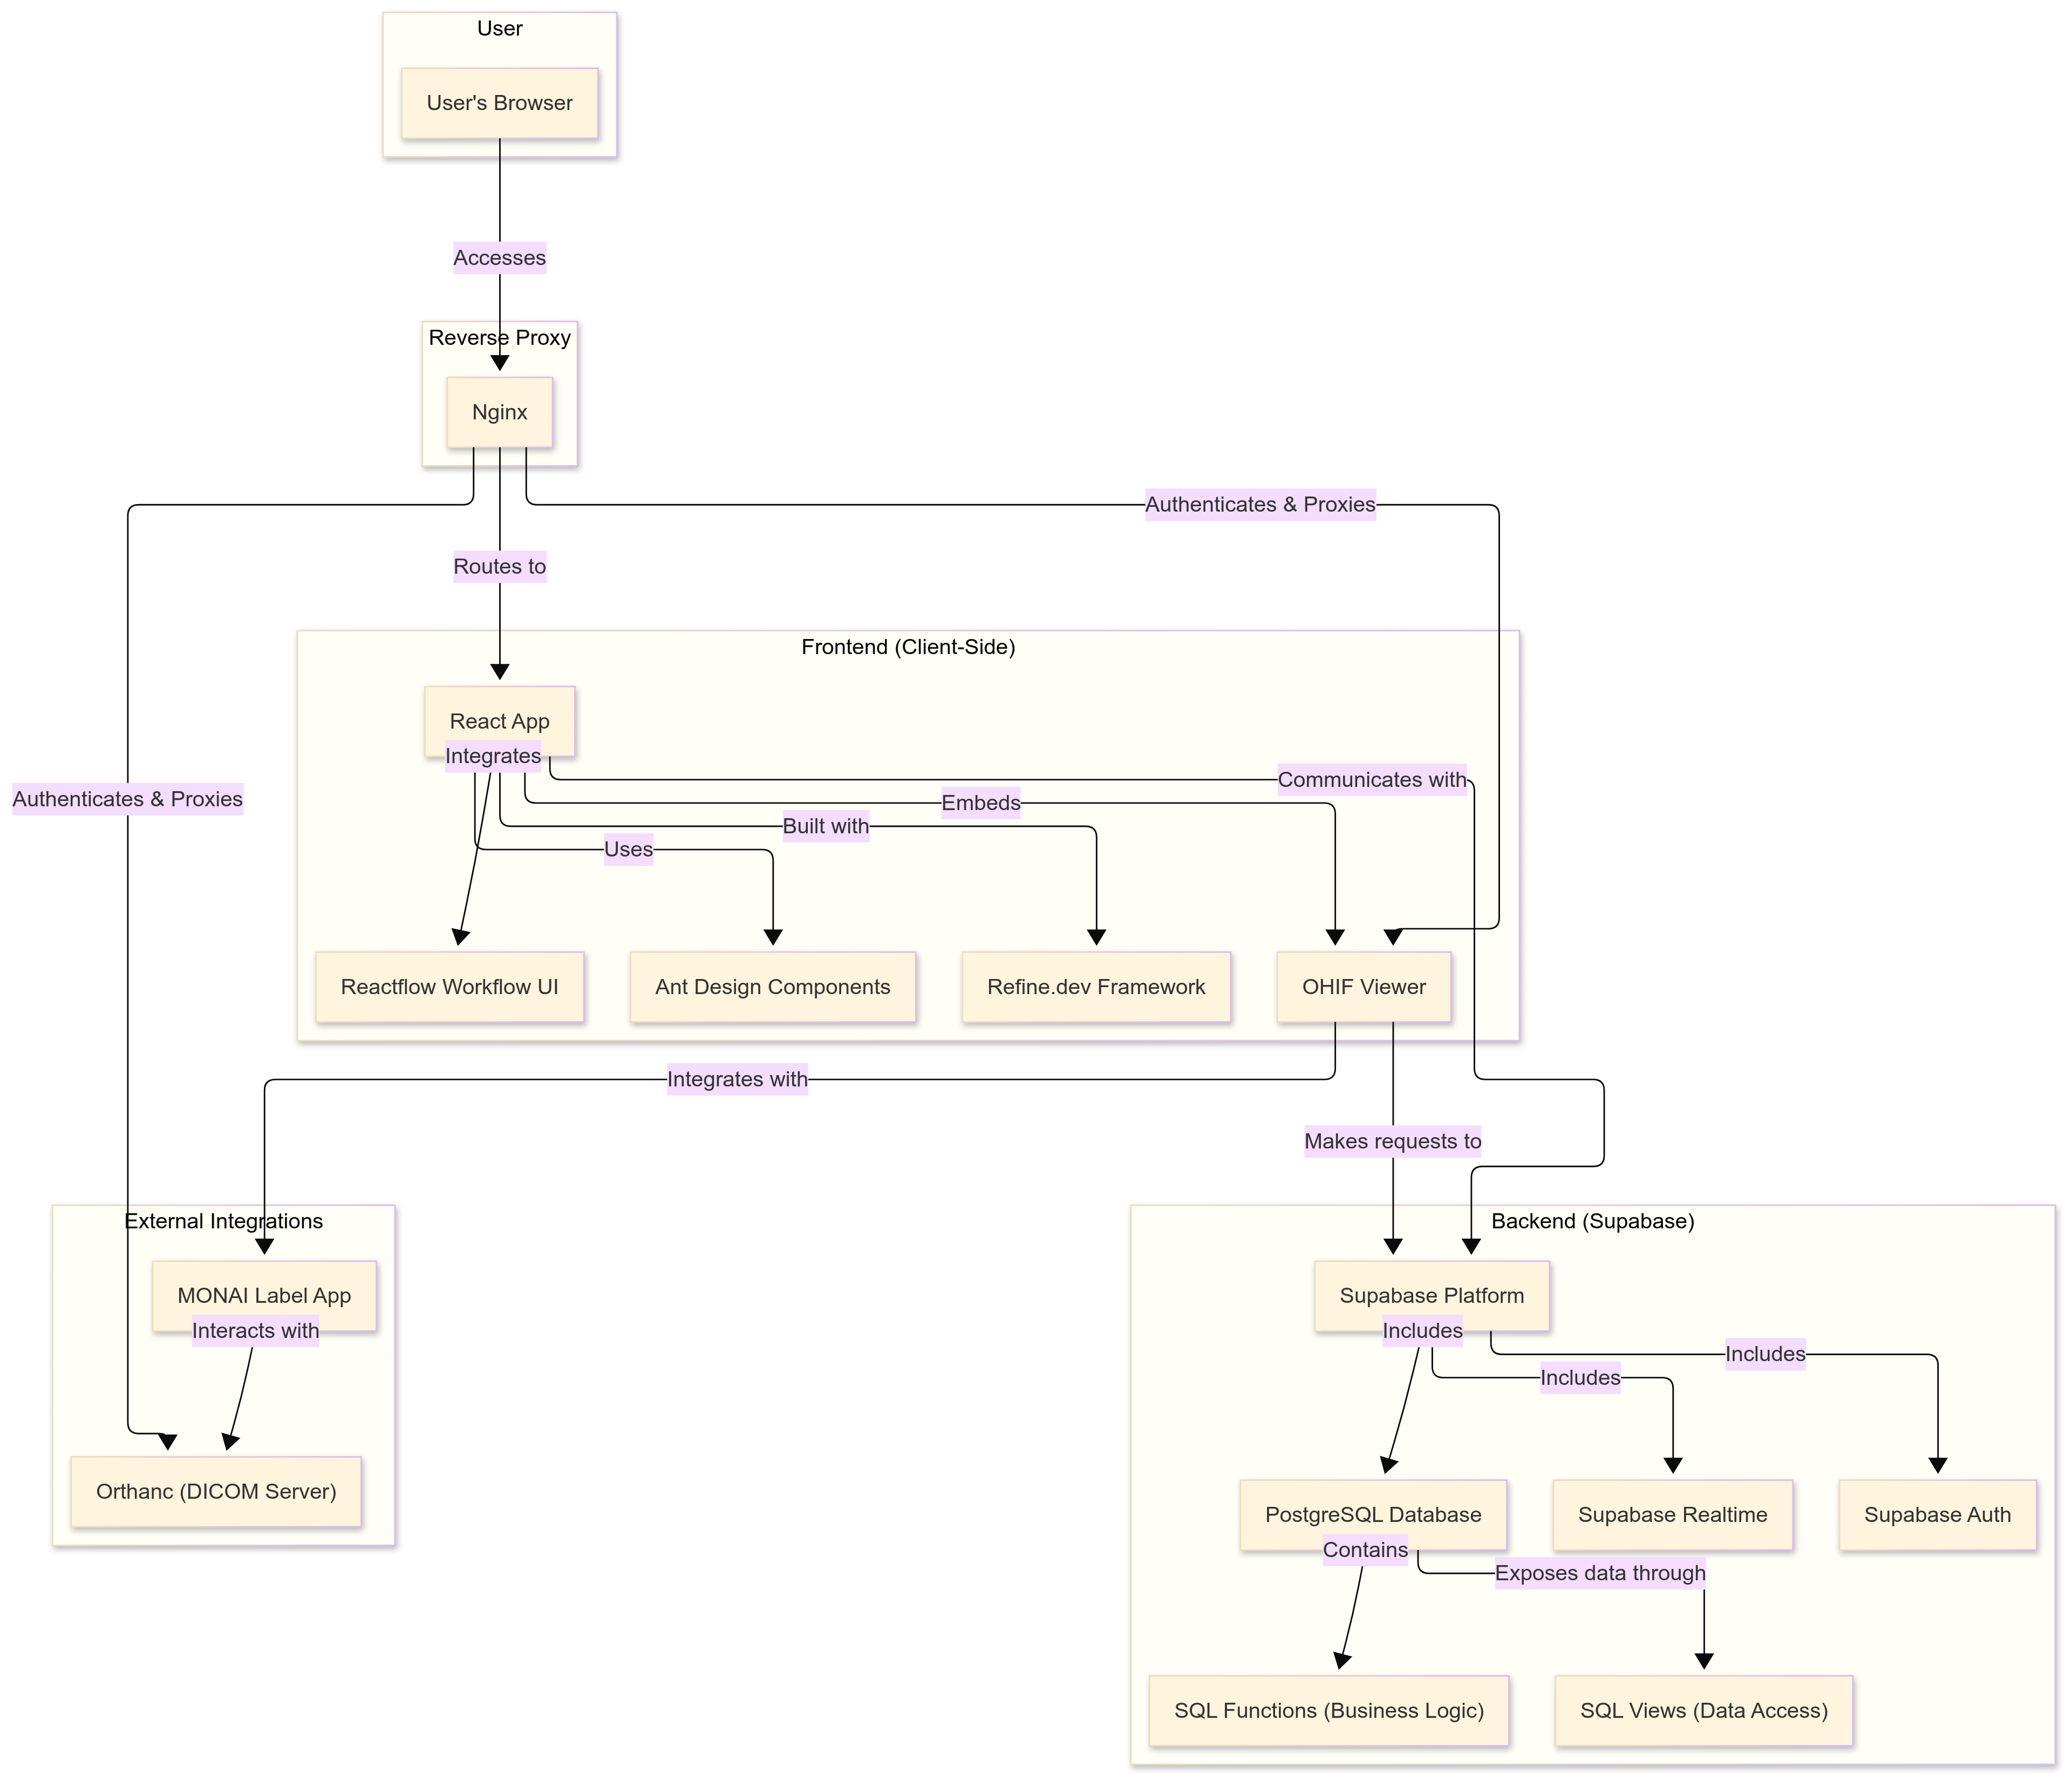
\includegraphics[width=\textwidth]{content/resources/images/system-architecture.md}
    \caption{High-Level System Architecture of the Intelligent Medical Annotation System}
    \label{fig:high-level-architecture}
\end{figure}

\textbf{Multi-Tier Architecture Design:} The system implements a multi-tier architecture with clear separation between presentation, business logic, and data management layers. This separation enables independent scaling and optimization of each layer based on specific performance requirements.

\textbf{Cloud-Native Design Principles:} The architecture follows cloud-native design principles, enabling deployment in various environments from on-premises healthcare data centers to public cloud platforms while maintaining consistent functionality and performance.

\textbf{Microservices Organization:} Each major system component is implemented as an independent microservice with well-defined interfaces and responsibilities. This organization enables independent development, testing, and deployment of system components.

\subsection{Data Flow Architecture}

The system implements a sophisticated data flow architecture that efficiently handles the movement and processing of medical imaging data throughout the annotation workflow.

\textbf{Medical Image Data Pipeline:} Medical images flow from source PACS systems through the Orthanc data management layer to the OHIF annotation interface. This pipeline includes automatic format conversion, metadata extraction, and performance optimization to ensure optimal user experience.

\textbf{Annotation Data Management:} Annotation data flows bidirectionally between the annotation interface and the workflow management system, enabling real-time collaboration and progress tracking while maintaining data consistency and version control.

\textbf{AI Integration Data Flow:} The AI assistance engine integrates into the data flow through standardized APIs that enable seamless transfer of image data for AI processing and return of AI-generated annotations to the user interface.

\textbf{Workflow Orchestration:} The workflow management platform orchestrates data flow between all system components based on defined workflow rules and user activities, ensuring that annotation tasks progress efficiently through defined stages.

\subsection{Integration Approach and Deployment Strategy}

The system is designed to support flexible deployment scenarios that accommodate various institutional requirements and technical constraints.

\textbf{Containerized Deployment:} All system components are containerized using Docker, enabling consistent deployment across different environments and simplifying system administration and maintenance.

\textbf{Scalable Infrastructure:} The architecture supports both vertical and horizontal scaling, allowing institutions to adjust system capacity based on user load and data volume requirements.

\textbf{Integration Gateway:} A centralized integration gateway manages communication between system components and external systems, providing a single point of control for system access and security policies.

\textbf{Progressive Deployment Strategy:} The system supports progressive deployment strategies that allow institutions to gradually migrate from existing annotation workflows to the new intelligent system, minimizing disruption and enabling thorough testing and validation.

This high-level architecture provides the foundation for the detailed system design and implementation that will be presented in the following chapters. The architecture ensures that the system can meet the identified requirements while providing flexibility for future enhancement and adaptation to evolving medical annotation needs. 